\section{Frequenzverhalten \tiny{$Revision: 996 $}}
\subsection{Logarithmische Darstellungen}
\begin{tabular}{ll}
\parbox{7cm}{
	\scriptsize
	\begin{tabular}{|c|c|c|c|}
	\hline
	\textbf{Lrel. (dB)} & \textbf{Lrel. (NP)} & \textbf{P2/P1} & \textbf{A2/A1} \\ \hline
	$100.000$ & $11.513$ & $10^{10}$ & $10^5$ \\ \hline
	$90.000$ & $10.362$ & $10^9$ & $31622.777$ \\ \hline
	$80.000$ & $9.210$ & $10^8$ & $10^4$ \\ \hline
	$70.000$ & $8.059$ & $10^7$ & $3162.278$ \\ \hline
	$60.000$ & $6.908$ & $10^6$ & $10^3$ \\ \hline
	$50.000$ & $5.756$ & $10^5$ & $316.228$ \\ \hline
	$40.000$ & $4.605$ & $10^4$ & $10^2$ \\ \hline
	$30.000$ & $3.454$ & $10^3$ & $31.623$ \\ \hline
	\textbf{$20.000$} & $2.303$ & \textbf{$10^2$} & \textbf{$10.000$} \\ \hline
	$19.085$ & $2.197$ & $81.000$ & $9.000$ \\ \hline
	$19.000$ & $2.187$ & $79.433$ & $8.913$ \\ \hline
	$18.062$ & $2.079$ & $64.000$ & $8.000$ \\ \hline
	$18.000$ & $2.072$ & $63.096$ & $7.943$ \\ \hline
	$17.000$ & $1.957$ & $50.119$ & $7.079$ \\ \hline
	$16.902$ & $1.946$ & $49.000$ & $7.000$ \\ \hline
	$16.000$ & $1.842$ & $39.811$ & $6.310$ \\ \hline
	$15.563$ & $1.792$ & $36.000$ & $6.000$ \\ \hline
	$15.000$ & $1.727$ & $31.623$ & $5.623$ \\ \hline
	$14.000$ & $1.612$ & $25.119$ & $5.012$ \\ \hline
	\textbf{$13.979$} & $1.609$ & \textbf{$25.000$} & \textbf{$5.000$} \\ \hline
	$13.000$ & $1.497$ & $19.953$ & $4.467$ \\ \hline
	\textbf{$12.041$} & $1.386$ & \textbf{$16.000$} & \textbf{$4.000$} \\ \hline
	\textbf{$12.000$} & $1.382$ & $15.849$ & $3.981$ \\ \hline
	$11.000$ & $1.266$ & $12.589$ & $3.548$ \\ \hline
	\textbf{$10.000$} & $1.151$ & \textbf{$10.000$} & $3.162$ \\ \hline
	$9.542$ & $1.099$ & $9.000$ & $3.000$ \\ \hline
	$9.000$ & $1.036$ & $7.943$ & $2.818$ \\ \hline
	$8.000$ & $0.921$ & $6.310$ & $2.512$ \\ \hline
	$7.000$ & $0.806$ & $5.012$ & $2.239$ \\ \hline
	\textbf{$6.021$} & \textbf{$0.693$} & \textbf{$4.000$} & \textbf{$2.000$} \\ \hline
	$6.000$ & $0.691$ & $3.981$ & $1.995$ \\ \hline
	$5.000$ & $0.576$ & $3.162$ & $1.778$ \\ \hline
	$4.000$ & $0.461$ & $2.512$ & $1.585$ \\ \hline
	\textbf{$3.010$} & \textbf{$0.347$} & \textbf{$2.000$} & \textbf{$1.414$} \\ \hline
	$3.000$ & $0.345$ & $1.995$ & $1.413$ \\ \hline
	$2.000$ & $0.230$ & $1.585$ & $1.259$ \\ \hline
	$1.000$ & $0.115$ & $1.259$ & $1.122$ \\ \hline
	$0.000$ & $0.000$ & $1.000$ & $1.000$ \\ \hline
	-$1.000$ & -$0.115$ & $0.794$ & $0.891$ \\ \hline
	-$2.000$ & -$0.230$ & $0.631$ & $0.794$ \\ \hline
	-$3.000$ & -$0.345$ & $0.501$ & $0.708$ \\ \hline
	-$4.000$ & -$0.461$ & $0.398$ & $0.631$ \\ \hline
	-$5.000$ & -$0.576$ & $0.316$ & $0.562$ \\ \hline
	-$6.000$ & -$0.691$ & $0.251$ & $0.501$ \\ \hline
	-$7.000$ & -$0.806$ & $0.200$ & $0.447$ \\ \hline
	-$8.000$ & -$0.921$ & $0.158$ & $0.398$ \\ \hline
	-$9.000$ & -$1.036$ & $0.126$ & $0.355$ \\ \hline
	-$10.000$ & -$1.151$ & $0.100$ & $0.316$ \\ \hline
	-$15.000$ & -$1.727$ & $0.032$ & $0.178$ \\ \hline
	-$20.000$ & -$2.303$ & $10^{-2}$ & $0.100$ \\ \hline
	-$30.000$ & -$3.454$ & $10^{-3}$ & $0.032$ \\ \hline
	-$40.000$ & -$4.605$ & $10^{-4}$ & $0.010$ \\ \hline
	-$50.000$ & -$5.756$ & $10^{-5}$ & $0.003$ \\ \hline
	-$60.000$ & -$6.908$ & $10^{-6}$ & $0.001$ \\ \hline
	-$70.000$ & -$8.059$ & $10^{-7}$ & $0.000$ \\ \hline
	-$80.000$ & -$9.210$ & $10^{-8}$ & $10^{-4}$ \\ \hline
	-$90.000$ & -$10.362$ & $10^{-9}$ & $3.162 \cdot 10^{-5}$ \\ \hline
	-$100.000$ & -$11.513$ & $10^{-10}$ & $10^{-5}$ \\ \hline
	\end{tabular}

	\normalsize
}
& \parbox{11.5cm}{
Verstärkungsmass L in \textbf{Dezibel} (dB):\\
$L_P = 10 \cdot \log \left(\frac {P_2} {P_1}\right)$ \\
$L_A = 20 \cdot \log \left(\frac {A_2} {A_1}\right)$ \\ 

Dezibel L zu linear: \\
$P_2 = P_1 \cdot 10^{\frac{L_P}{10}} $ \\
$A_2 = A_1 \cdot 10^{\frac{L_A}{20}} $ \\

Verstärkungsmass L in \textbf{Neper} (Np):\\
$L_P = \frac {1}{2} \cdot \ln \left(\frac {P_2} {P_1}\right)$\\
$L_A = \ln \left(\frac {A_2} {A_1} \right)$ \\

Neper zu linear: \\
$P_2 = P_1 \cdot e^{2 L_P}$ \\
$A_2 = A_1 \cdot e^{L_A}$ \\

Die Umrechnung zwischen {\bf dB} und {\bf Np} ist linear: \\
$1\mbox{~dB} = \frac {\ln(10)} {20} \mbox{~Np} = 0.1151\mbox{~Np}$ \\
$1\mbox{~Np} = 20 \cdot \log(\mbox{e}) \mbox{~dB} = 8.686\mbox{~dB}$ \\ 
\\
Anstatt $\frac{X_2}{X_1}$ für Verstärkungsmasse ($L$) können auch
$\frac{X_1}{X_2}$ für Dämpfungsmasse ($a$) verwendet werden!

\small{($P$ für Leistungen, $A$ für Amplituden)}
\\ \\ \\

\textbf{Hilfen zur Berechnung}\\
\begin{tabular}{|l|ll|}
\hline
$x Db$	& $L_P=P_2/P_1$ &$L_A=A_2/A_1$ \\
\hline
$-x dB$	& $1/L_P$	& $1/L_A$\\
$x+3dB$	& $L_P \cdot 2$	& $L_A \cdot \sqrt{2} \approx L_A \cdot 1.414$ \\
$x+10dB$	& $L_P \cdot 10$ & $L_A \cdot \sqrt{10} \approx L_A \cdot 3.162$\\
\hline
\end{tabular}
\\ \\ \\

\textbf{Relative \& absolute Pegel}\\
Relativer Pegel: Pegel relativ zu definiertem Wert\\
Absoluter Pegel: Pegel an Normgenerator ($R_i = 600 \Omega$, $1mW$ Leistung am
Widerstand)\\ 
\begin{tabular}{|l|l|l|}\hline
  & dBu & Spannungspegel bezogen auf 774.6~mV an 600~$\Omega$\\ \cline{2-3}
 \multicolumn{1}{|l|}{\raisebox{1.5ex}[-1.5ex]{$\mbox{dB}_{abs.}$}} & dBm & Leistungspegel bezogen auf 1~mW an 600~$\Omega$\\ \hline\hline
  & dBV & Spannungspegel bezogen auf 1~V\\ \cline{2-3}
  & dB$\mu$V & Spannungspegel bezogen auf 1~$\mu$V\\ \cline{2-3}
  & dBf & Leistungspegel bezogen auf $10^{-15}$~W\\ \cline{2-3} 
\multicolumn{1}{|l|}{$\mbox{dB}_{rel.}$}  & dBW & Leistungspegel bezogen auf 1~W\\ \cline{2-3}
  & dBk & Leistungspegel bezogen auf 1~kW\\ \cline{2-3}
  & dBr & relativer Pegel\\ \cline{2-3}
  & dB0 & Pegel auf 0~dB bezogen\\ \hline
\end{tabular}\\

}
\end{tabular}
\newpage

\subsection{Minimal- und nicht-minimalphasige Systeme}
\subsubsection{Allpass-Systeme}
Allpässe werden vor allem als Laufzeitkorrekturglieder und als
Verzögerungselemente verwendet. Der Amplitudengang ist konstant ($|H(jw)| =
const \neq 0$) und die Pol- bzw. Nullstellen haben in Paaren auftretende Null-
und Polstellen, die symmetrisch zu $j \omega$-Achse liegen. Dabei liegen die
Nullstellen auf der RHE.
UTF: $T_A(s) = K
\frac{Q(-s)}{Q(s)}$


\subsubsection{Minimalphasennetzwerk}
Ein Minimalphasennetzwerk hat \textbf{keine Nullstellen in der rechten
Halbebene} (RHE), \textbf{darf jedoch Nullstellen auf der imaginären Achse
haben}.

\subsubsection{Nicht-Minimalphasennetzwerk}
Ein Nicht-Minimalphasennetzwerk kann durch Kaskadierung eines Allpasses und
eine Minimalphasennetzwerk realisiert werden:\\
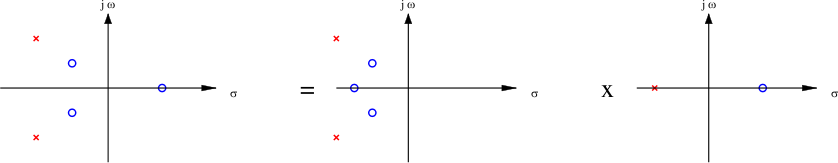
\includegraphics[width=12cm]{./bilder/nicht-minimalphasennetzwerk.png}\\
Nicht-Minimalphasennetzwerk (links) = Minimalphasennetzwerk (Mitte) · Allpass (rechts)

\subsection{Stabilitätsbestimmung am Pol-/Nullstellendiagramm}
asymptotisch stabil = alle Polstellen in der
linken Halbebene (LHE)\\
grenzstabil=Polstellen in der LHE und/oder auf der
imaginären Achse

\subsection{Bode-Diagramm \matlab{bode}}
\begin{tabular}{ll}
	\parbox{7cm}{
		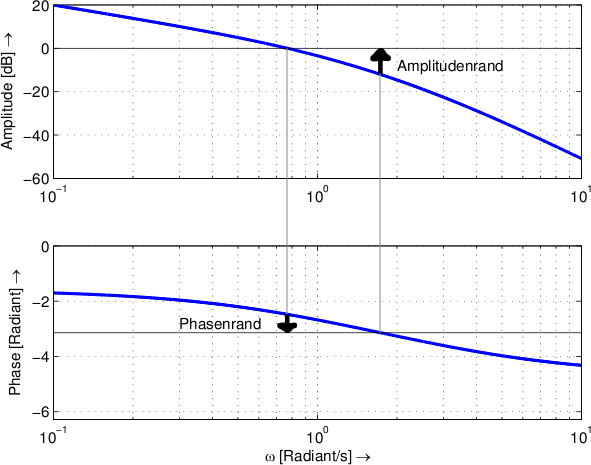
\includegraphics[width=7cm]{./bilder/bode-stabilitaet.png}
	}
	& \parbox{11cm}{
		\subsubsection{Definition}
		Das Bodediagramm besteht aus zwei Graphen, einer zeigt die Amplitude in
		doppelt-logarithmischer Form, der zweite zeigt die Phase in Grad und in
		linearer Form in Abhängigkeit der Frequenz dar.
		
		\subsubsection{Stabilitätsbestimmung \formelbuch{210} \matlab{margin,
		allmargin}}
		Der {\bf Amplitudenrand} ist der Abstand des
		Amplitudenganges zur 0~dB-Linie bei der Kreisfrequenz $\omega$, wo die Phase
		gleich $-\pi$ (-180 Grad) ist. \\
		
		Der {\bf Phasenrand} ist der Abstand das Phasenganges zur
		-$\pi$-Linie bei der Kreisfrequenz $\omega$, wo die Amplitude gleich 0~dB
		ist. \\
		
		Damit eine System stabil ist, m\"ussen Phasen- und Amplitudenrand
		$>0$ sein. Je gr\"osser der Phasen- und Amplitudenrand ist, desto
		``stabiler'' ist das System.
	}
\end{tabular}

\newpage 
\subsubsection{Approximation des Bode-Diagramms \formelbuch{193}}
\renewcommand{\arraystretch}{1.5}
\begin{tabular}{|p{4cm}|p{1.2cm}p{5cm}|p{1.2cm}p{4.5cm}|}
\hline
\textbf{UTF $H(s)$}
	& \textbf{Amplitude $|H(s)|$}
	&
	& \textbf{Phase $ \angle(H(s))$}
	& \\
\hline
\hline
1) Konstanter Faktor & & & & \\
	$\alpha e^{j \beta}$
	& \parbox{1cm}{
		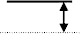
\includegraphics[width=1cm]{./bilder/bode-approx-konst.png}
	} 
	& Konst. $20 \log \alpha$
	& \parbox{1cm}{
		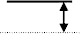
\includegraphics[width=1cm]{./bilder/bode-approx-konst.png}
	} 
	& Konst. $\beta$ \\
\hline
2) Pol im Ursprung & & & &\\
	$\frac{\alpha}{s}$
	& \parbox{1cm}{
		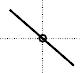
\includegraphics[width=1cm]{./bilder/bode-approx-ampl-tp-ord1.png}
	} 
	& \parbox{5cm}{
		Lin. Steigung $-20 db/Dek.$\\
		$0dB$ bei $\omega = \alpha$
	}
	& \parbox{1cm}{
		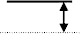
\includegraphics[width=1cm]{./bilder/bode-approx-konst.png}
	} 
	& Konst. $-\frac{\pi}{2}$ \\
\hline
3) Nullstelle im Ursprung & & & &\\
	$\alpha s$
	& \parbox{1cm}{
		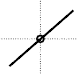
\includegraphics[width=1cm]{./bilder/bode-approx-ampl-hp-ord1.png}
	} 
	& \parbox{5cm}{
		Lin. Steigung $+20 db/Dek.$\\
		$0dB$ bei $\omega = \frac{1}{\alpha}$
	}
	& \parbox{1cm}{
		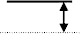
\includegraphics[width=1cm]{./bilder/bode-approx-konst.png}
	} 
	& Konst. $+\frac{\pi}{2}$ \\
\hline
4a) Reeller Pol & & & &\\
	$\frac{1}{s + \alpha}$
	& \parbox{1cm}{
		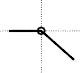
\includegraphics[width=1cm]{./bilder/bode-approx-ampl-4.png}
	} 
	& \parbox{5cm}{
		Konst. $-20 \log \alpha$ für $\omega < \alpha$\\
		dann Steigung $-20dB/Dek.$ 
	}
	& \parbox{1cm}{
		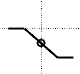
\includegraphics[width=1cm]{./bilder/bode-approx-phase-4.png}
	} 
	& \parbox{4.5cm}{
		Konst. $0$ für $\omega < \frac{\alpha}{10} $\\
		Konst. $-\frac{\pi}{2}$ für $\omega > 10 \alpha$
	}\\
\hline
4b) Reeller Pol &&&&\\
	$\frac{\alpha}{s + \alpha}$
	& \parbox{1cm}{
		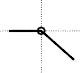
\includegraphics[width=1cm]{./bilder/bode-approx-ampl-4.png}
	} 
	& \parbox{5cm}{
		Konst. $0dB$ für $\omega < \alpha$\\
		dann Steigung $-20dB/Dek.$
	}
	& \parbox{1cm}{
		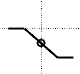
\includegraphics[width=1cm]{./bilder/bode-approx-phase-4.png}
	} 
	& \parbox{4.5cm}{
		Konst. $0$ für $\omega < \frac{\alpha}{10} $\\
		Konst. $-\frac{\pi}{2}$ für $\omega > 10 \alpha$
	}\\
\hline
5a) Reelle Nullstelle &&&& \\
	$s + \alpha$
	& \parbox{1cm}{
		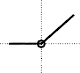
\includegraphics[width=1cm]{./bilder/bode-approx-ampl-5.png}
	} 
	& \parbox{5cm}{
		Konst. $20 \log \alpha$ für $\omega < \alpha$\\
		dann Steigung $+20dB/Dek.$
	}
	& \parbox{1cm}{
		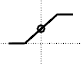
\includegraphics[width=1cm]{./bilder/bode-approx-phase-5.png}
	} 
	& \parbox{4.5cm}{
		Konst. $0$ für $\omega < \frac{\alpha}{10} $\\
		Konst. $+\frac{\pi}{2}$ für $\omega > 10 \alpha$
	}\\
\hline
5b) Reelle Nullstelle &&&& \\
	$\frac{s + \alpha}{\alpha}$
	& \parbox{1cm}{
		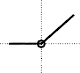
\includegraphics[width=1cm]{./bilder/bode-approx-ampl-5.png}
	} 
	& \parbox{5cm}{
		Konst. $0dB$ für $\omega < \alpha$\\
		dann Steigung $+20dB/Dek.$
	}
	& \parbox{1cm}{
		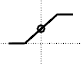
\includegraphics[width=1cm]{./bilder/bode-approx-phase-5.png}
	} 
	& \parbox{4.5cm}{
		Konst. $0$ für $\omega < \frac{\alpha}{10} $\\
		Konst. $+\frac{\pi}{2}$ für $\omega > 10 \alpha$
	}\\
\hline
\multicolumn{2}{|l}{6a) Konjugiert-komplexe Pole} &&& \\
	$\frac{1}{s^2+s\frac{\omega_p}{q_p}+\omega_p^2}$
	& \parbox{1cm}{
		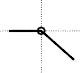
\includegraphics[width=1cm]{./bilder/bode-approx-ampl-6.png}
	} 
	& \parbox{5cm}{
		Konst. $-40 \log \omega_p$ für $\omega < \omega_p$\\
		dann Steigung $-40dB/Dek.$ für $\omega > \omega_p; -40 \log \omega_p$\\
		Überhöhung zwischen $\frac{\omega_p}{2}$, $\omega_p$ \& $2 \omega_p$\\
		Max. $20 \log \frac{q_p}{\omega_p^2}$ bei $\omega = \omega_p$
		}
	& \parbox{1cm}{
		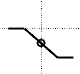
\includegraphics[width=1cm]{./bilder/bode-approx-phase-6.png}
	} 
	& \parbox{4.5cm}{
		Konst. $0$ für $\omega < \frac{\omega_p}{10^{\frac{1}{2q_p}}} $\\
		Konst. $-\pi$ für $\omega > \omega_p 10^{\frac{1}{2q_p}}$\\
		$-\frac{\pi}{2}$ bei $\omega = \omega_p$
	}\\
\hline
\multicolumn{2}{|l}{6b) Konjugiert-komplexe Pole} &&& \\
	$\frac{\omega_p^2}{s^2+s\frac{\omega_p}{q_p}+\omega_p^2}$
	& \parbox{1cm}{
		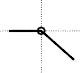
\includegraphics[width=1cm]{./bilder/bode-approx-ampl-6.png}
	} 
	& \parbox{5cm}{
		Konst. $0dB$ für $\omega < \omega_p$\\
		dann Steigung $-40dB/Dek.$ für $\omega > \omega_p; 0dB$\\
		Überhöhung zwischen $\frac{\omega_p}{2}$, $\omega_p$ \& $2 \omega_p$,
		Max. $20 \log q_p$ bei $\omega = \omega_p$
		}
	& \parbox{1cm}{
		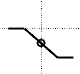
\includegraphics[width=1cm]{./bilder/bode-approx-phase-6.png}
	} 
	& \parbox{4.5cm}{
		Konst. $0$ für $\omega < \frac{\omega_p}{10^{\frac{1}{2q_p}}} $\\
		Konst. $-\pi$ für $\omega > \omega_p 10^{\frac{1}{2q_p}}$\\
		Bei $\omega = \omega_p$ genau $-\frac{\pi}{2}$
	}\\
\hline
\multicolumn{2}{|l}{7) Konjugiert-komplexe Nullstellen} &&& \\
	\parbox{4cm}{
		$s^2+s\frac{\omega_z}{q_z}+\omega_z^2$ \\ bzw. \\
		$\frac{s^2+s\frac{\omega_z}{q_z}+\omega_z^2}{\omega_z^2}$
	}
	& \multicolumn{2}{|l|}{
		\parbox{6.2cm}{
		Analog zu 6a, 6b (jedoch Spiegelung an der 0dB-Linie)}
	}
	
	& \multicolumn{2}{|l|}{
		\parbox{6.2cm}{Analog zu 6a, 6b (jedoch Spiegelung an der 0 Grad-Linie)}
	}\\
\hline
\multicolumn{5}{|l|}{
	\parbox{18cm}{
	8) Serieschaltung von Systemen erfolgt durch \textbf{Superposition} der
	einzelnen Bode-Diagramme (Multiplikation von UTFs entspricht Addition im
	dB-Bereich). } } \\

\hline
\end{tabular}
\renewcommand{\arraystretch}{1}

\textbf{Werte für $q_p$ bzw. $q_z$}\\
\renewcommand{\arraystretch}{1.5}
\begin{tabular}{|r|r|r||r|r|r||r|r|r||r|r|r||r|r|r|}
\hline
\multicolumn{1}{|l|}{$q$} & \multicolumn{1}{l|}{$10^{\frac{1}{2 q_p}}$} & 
\multicolumn{1}{l||}{$\frac{1}{10^{\frac{1}{2 q_p}}}$} &
\multicolumn{1}{l|}{$q$} & \multicolumn{1}{l|}{$10^{\frac{1}{2 q_p}}$} &
\multicolumn{1}{l||}{$\frac{1}{10^{\frac{1}{2 q_p}}}$} &
\multicolumn{1}{l|}{$q$} & \multicolumn{1}{l|}{$10^{\frac{1}{2 q_p}}$} & \multicolumn{1}{l||}{$\frac{1}{10^{\frac{1}{2 q_p}}}$} & \multicolumn{1}{l|}{$q$} & \multicolumn{1}{l|}{$10^{\frac{1}{2 q_p}}$} & \multicolumn{1}{l||}{$\frac{1}{10^{\frac{1}{2 q_p}}}$} & \multicolumn{1}{l|}{$q$} & \multicolumn{1}{l|}{$10^{\frac{1}{2 q_p}}$} & \multicolumn{1}{l|}{$\frac{1}{10^{\frac{1}{2 q_p}}}$} \\ \hline
\hline
1 & 3.162 & 0.316 & 5 & 1.259 & 0.794 & 9 & 1.136 & 0.880 & 13 & 1.093 & 0.915 & 17 & 1.070 & 0.935 \\ \hline
2 & 1.778 & 0.562 & 6 & 1.212 & 0.825 & 10 & 1.122 & 0.891 & 14 & 1.086 & 0.921 & 18 & 1.066 & 0.938 \\ \hline
3 & 1.468 & 0.681 & 7 & 1.179 & 0.848 & 11 & 1.110 & 0.901 & 15 & 1.080 & 0.926 & 19 & 1.062 & 0.941 \\ \hline
4 & 1.334 & 0.750 & 8 & 1.155 & 0.866 & 12 & 1.101 & 0.909 & 16 & 1.075 & 0.931 & 20 & 1.059 & 0.944 \\ \hline
\end{tabular}
\renewcommand{\arraystretch}{1}

\newpage
\subsection{Ortskurve (Nyquist-Diagramm) \formelbuch{198} \matlab{nyquist}}
\begin{tabular}{ll}
	\parbox{7cm}{
		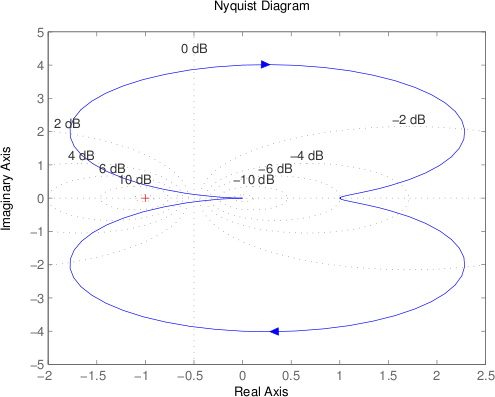
\includegraphics[width=7cm]{./bilder/nyquist.png}
	}
	& \parbox{11cm}{
		\subsubsection{Definition}
		Im Gegensatz zum Bode-Diagramm wird beim Nyquist-Diagramm Betrag und Phase in
		einem einzigen Diagramm dargestellt, nämlich indem man den Real- und
		Imaginärteil des Ausgabewertes direkt in die komplexe Zahlenebene zeichnet.
		
		\subsubsection{Stabilitätsbestimmung}
		Ist der {\bf offene} Regelkreis $H(s)$ {\bf asymptotisch
		stabil}\index{asymptotisch stabil}, so ist der {\bf geschlossene}
		Regelkreis $1+H(s)=D(s)+N(s)$ asymptotisch stabil, wenn die {\bf
		Ortskurve} des {\bf offenen} Regelkreises den kritischen Punkt
		(-1,$j0$) weder umkreist noch durchl\"auft.
	}
\end{tabular}


\subsection{Nichols-Diagramm \formelbuch{203} \matlab{nichols}}
\begin{tabular}{ll}
	\parbox{7cm}{
		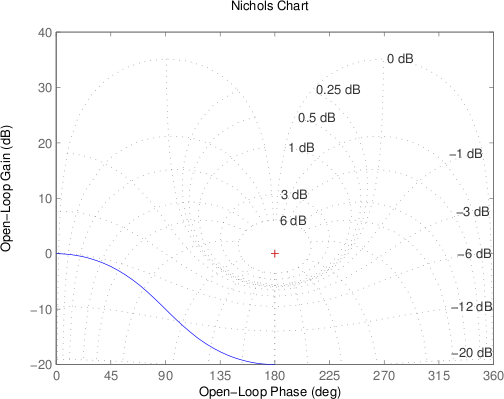
\includegraphics[width=7cm]{./bilder/nichols.png}
	}
	& \parbox{11cm}{
		\subsubsection{Definition}
		Das Nichols Diagramm (auch Amplituden-Phasen-Diagramm) ist die Darstellung des
		Absolutbetrages (Verstärkung, logarithmisch) in Abhängigkeit der Phase. Das Nichols Diagramm ist zur
		Bestimmung der Stabilität in rückgekoppelten Systemen verwendbar.
	}
\end{tabular}
